\documentclass[a4paper, 11pt, nofootinbib]{book}

\setcounter{tocdepth}{3}
\setcounter{secnumdepth}{3}
\usepackage{amsmath}
\usepackage{comment} % enables the use of multi-line comments (\ifx \fi) 
\usepackage{lipsum} %This package just generates Lorem Ipsum filler text. 
\usepackage{fullpage} % changes the margin
\usepackage[utf8]{inputenc}
\usepackage{gensymb}
\usepackage{graphicx}
\usepackage{booktabs}% http://ctan.org/pkg/booktabs
\usepackage{makecell}
\usepackage{tabularx}
\usepackage[table]{xcolor}
\usepackage{array}
\usepackage{wrapfig}
\usepackage{subcaption}
\usepackage{csquotes}
\usepackage{lscape}
\usepackage{afterpage}
\usepackage{geometry}
\usepackage{listings}
\usepackage{xcolor}
\usepackage{ulem}
\usepackage{chngcntr}
\usepackage{multicol}

%Tabellenheadings
\renewcommand*{\thead}[1]{\bfseries #1}

%Ermöglicht bullet-points in Tabellen
\newcommand \tabitem{\makebox[1em][r]{\textbullet~}}

%Abbildungen werden pro Kapitel nummeriert (Abb. 1.4, Abb. 4.7 etc)
\counterwithin{figure}{section}

\geometry{a4paper, margin=1in}

%Bilder haben die Unterschrift Abb. anstelle von Figure
\renewcommand{\figurename}{Fig..}

%\code{Text} formatiert Text als monospace Schrift
\newcommand{\code}[1]{\texttt{#1}}


%Wie sollen Code-Snippets mit \lstinline|code| aussehen?
\lstset{frame=tblr,
	captionpos=b,
	language=c,
	aboveskip=3mm,
	belowskip=3mm,
	showstringspaces=false,
	columns=flexible,
	basicstyle={\small\ttfamily},
	numbers=left,
	numberstyle=\tiny\color{gray},
	keywordstyle=\color{blue},
	commentstyle=\color{darkgreen},
	stringstyle=\color{violet},
	breaklines=true,
	breakatwhitespace=true,
	tabsize=3
}

%RGB-Definition von eiigen Farben
\definecolor{system}{RGB}{141,0,76}
\definecolor{inhalt}{RGB}{2,47,99}
\definecolor{darstellung}{RGB}{116,117,117}
\definecolor{nutzung}{RGB}{207,2,127}
\definecolor{darkgreen}{RGB}{39,117,1}

\begin{document}
\title{Summary Micro-Controller FS18}
\author{Alex Neher}
\maketitle

\tableofcontents

\graphicspath{{./Pictures/}}

\mainmatter
\chapter{Microcontroller}
\section{Components}
Micro controllers are so called \textbf{Single Chip} Computer, meaning everything is on a single PCB, as opposed to e.g. a 'normal' PC.

\begin{wrapfigure}[8]{R}{0.5\textwidth}
	\centering
	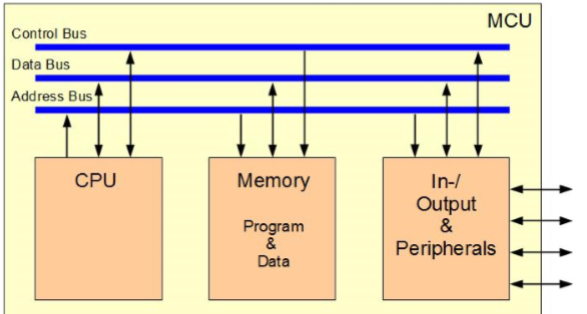
\includegraphics[keepaspectratio=true,height=10\baselineskip]{architecture.PNG}
	\caption{Von-Neumann Architecture}
	\label{fig:arch}
\end{wrapfigure}

MC consist of at least four components:

\begin{description}
	\item[CPU: ] Central Processing Unit
	\item[Memory: ] Where programs and data are stored
	\item[IO/Input-Output: ] Communication with Peripherals
	\item[Bus-System: ] Connects the components
\end{description}

\vspace{10px}

\noindent There are two different architectures:

\begin{description}
	\item[Von-Neumann: ] One shared bus for program and data. Program and data are in the same memory. Often found in low-cost MCs
	\item[Harvard: ] Two separate bus systems for program and data. Often found in high-performance MCs
\end{description}
\vspace{10px}

\noindent Usually, a read/write-operation goes through four steps:

\begin{enumerate}
	\item CPU puts the address on the address bus
	\item Either the memory or the IO claim the address as their
	\item CPU tells the component via the control bus whether the operation is read or write
	\item 
		\subitem \textit{read: } The memory or IO places the data of the requested address on the data bus
		\subitem \textit{write: } The CPU writes the data on the mentioned address via data bus
\end{enumerate}

\section{Numerical systems}
In MC, variables and constants are seldom stored as decimal value. Rather they're either stored as a binary or a hexadecimal value. 

In general, mathematical terms an $n$-digit integer to the base $B$ can be expressed as:

\[ \scalebox{1.5}{$ \sum_{i=0}^{n-1} x_{i} * B^i = X_{0} * B^0 + x_{1} * B^2 + [...] + x_{n-1} * B^{n-1} $} \]

\noindent Or easier: \textit{Multiply the $n$-th digit of the integer with $B^{n-1}$ starting from the right} with n = 0

\subsection{Example}

\noindent $1100'0101_{2}$ (binary) to decimal \\
$
	= 1*2^0 + 0*2^1 + 1*2^2 + 0*2^3 + 0*2^4 + 0*2^5 + 1*2^6 + 1*2^7 \\
	=   1   +   0   +   4   +   0   +   0   +  0   +   64   +  128 \\
	=   \underline{\underline{197_{10}}}
$

\noindent If you have to convert a number between two 'exotic' systems, say base 8 to base 3, it's usually easier to convert it to decimal first and then convert it to the desired system again ($x_{8} \rightarrow x_{10} \rightarrow x_{3}$). An exception to that is binary to hexadecimal and vice versa. One digit in hexadecimal represents four digits in binary, so you can directly convert blocks of four:

\noindent $1100'0101_{2}$ to hexadecimal:
\vspace{10px}

\noindent
$1100 = 0*2^0 + 0* 2^1 + 1*2^2 + 1*2^3 = 0 + 0 + 4 + 8 = 12_{10} = C_{16} \\
0101 = 1 * 2^0 + 0*2^1  + 1*2^2 + 0*2^3 = 1 + 0 + 4 + 0 = 5_{10} = 5_{16} \\
\rightarrow 1100'0101_{2} = C5_{16}
$

\subsection{Two's Complement}
Especially in MC-technology, signed numbers (that can also be negative) are mostly stored as \textit{two's complement}. You basically take the binary number, invert every digit and add one. So -28 would be stored as
\vspace{10px}

\noindent
$ 28_{10} = 16 + 8 + 4 = 2^2 + 2^3 + 2^4 = 0001'1100_{2}$ \\
invert \\
$ 0001'1100 \rightarrow 1110'0011$\\
add one \\
$1110'0011 + 1 = \underline{\underline{1110'0100}}$

\section{Logic Gates}
\begin{figure}[htb]
	\centering
	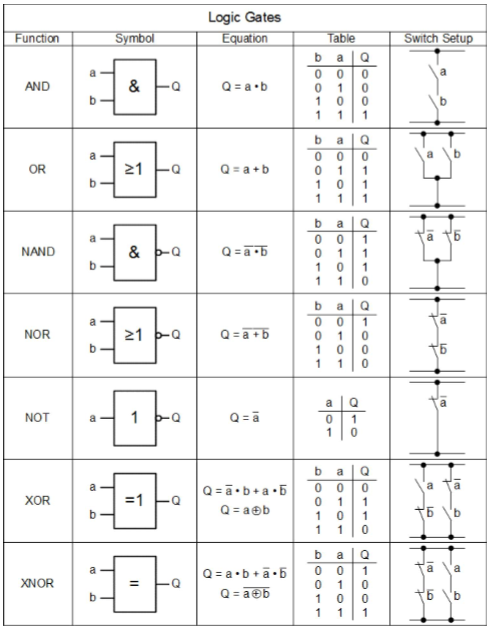
\includegraphics[keepaspectratio=true,height=25\baselineskip]{logicGates.PNG}
	\caption{Fundamental logic-Gates used in MCs}
	\label{fig:logicGates}
\end{figure}

\begin{figure}[htb]
	\centering
	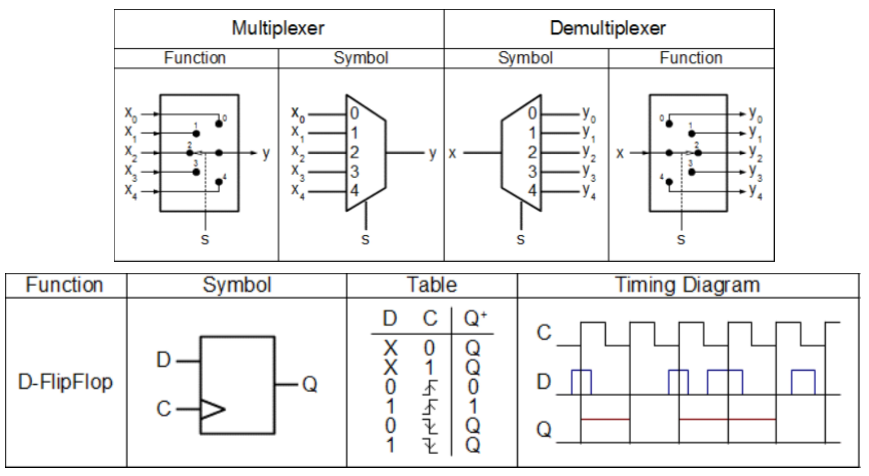
\includegraphics[keepaspectratio=true,height=15\baselineskip]{flipflop.PNG}
	\caption{Visualisation of the (de)multiplexer and the flipflop}
	\label{fig:multFlip}
\end{figure}

\begin{description}
	\item[Multiplexer: ] The multiplexer is a combinational logic circuit, which allows us to select one of many input lines and route it to the single, common output line. The demultiplier does the exact opposite: it takes one input and you can select to which output line it is routed
	\item[FlipFlop: ] Idunno %TODO: Get WTF FlipFlops are
\end{description}

\section{Instruction Set Cycle}

\begin{wrapfigure}[7.5]{L}{0.5\textwidth}
	\centering
	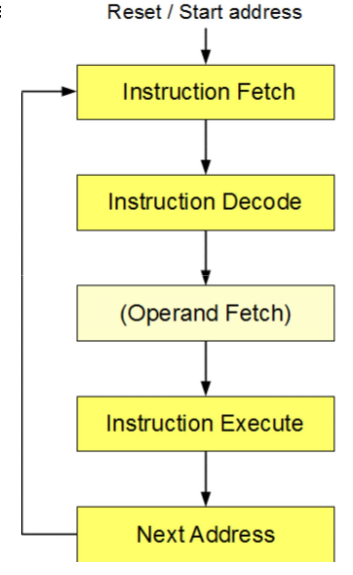
\includegraphics[keepaspectratio=true,height=20\baselineskip]{instructionCycle.PNG}
	\caption{Visualisation of the Instruction Set Cycle}
	\label{fig:instCycle}
\end{wrapfigure}

The way a CPU executes instructions can be shortened to \textbf{FDE}. It stands for \textbf{F}etch, \textbf{D}ecode \textbf{E}xecute. 
\vspace{10px}
S
\noindent As can be seen in fig. \ref{fig:instCycle}, the CPU first fetches the instruction from the memory, then it decodes it and decides if it has to fetch a second operand (e.g. for an addition). Afterwards it executes said instruction and moves on to the next address.


\newpage

\section{Assembler}
\subsection{Directives}
Put simply, Assembler directives are instructions that direct the assembler to do something:
\begin{center}
\begin{tabular}{|p{2cm}|p{5cm}|p{4cm}|p{5cm}|}
	\hline
	\thead{Directive} & \thead{Description} & \thead{Example} & \thead{Explanation} \\
	\hline
	SECTION & Defines the beginning of a relocatable section & ConstSec: SECTION & Puts the whole ConstSec-Section in the same RAM-section\\
	\hline
	EQU & Assign an expression to a name. Not redefinable & MaxElement: EQU 20 & search-and-replace every \textit{MaxElement} in the code with 20\\
	\hline
	DC & Defines one or more constants and theirnames & DC B \$AA & Pointer to address \$AA at every \textit{Alarm}\\
	\hline
	DS & Allocates memory to variables & DS W 3 & Reserves 3 words of RAM. 1 Word = 2 Bytes\\
	\hline
\end{tabular}
\end{center}

\subsection{Addressing modes}
There are six different addressing modes that are supported by our CPU:

\begin{description}
	\item[Immediate: ] 1 Byte operand in the instruction \\
		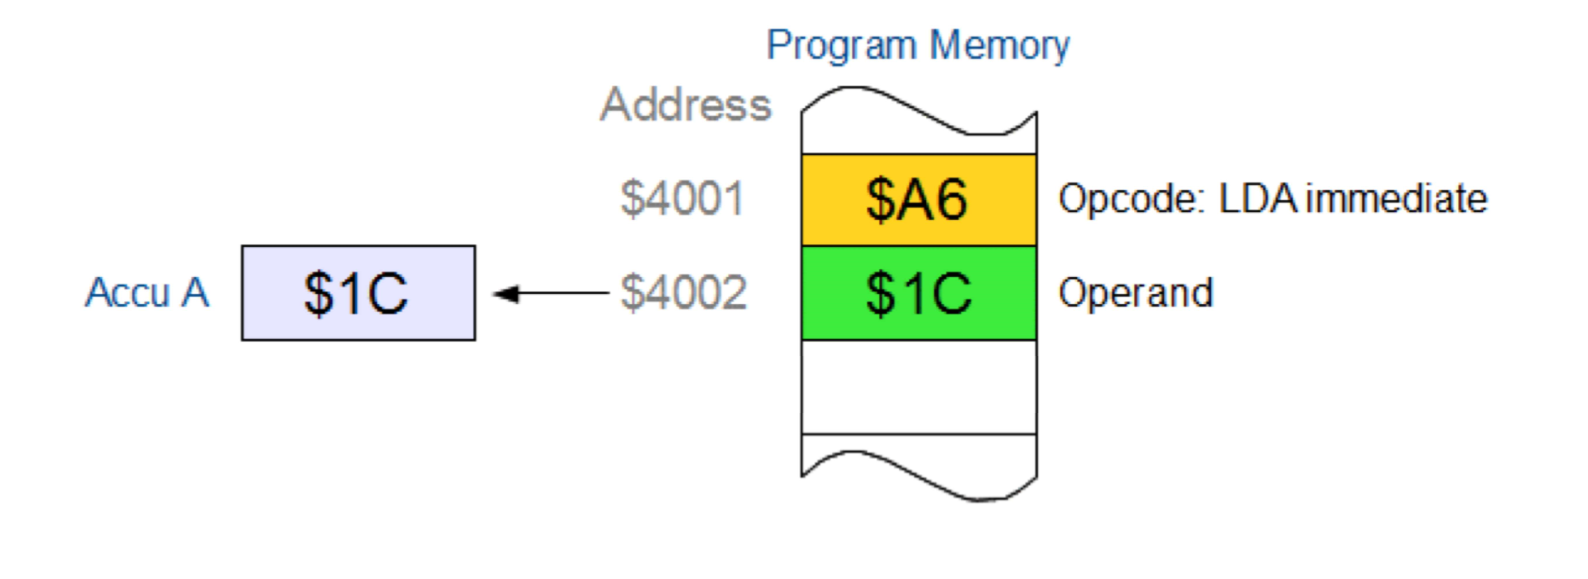
\includegraphics[keepaspectratio=true, height=10\baselineskip]{immAdd.PNG}
	\item[Inherent: ] No operand required \\
		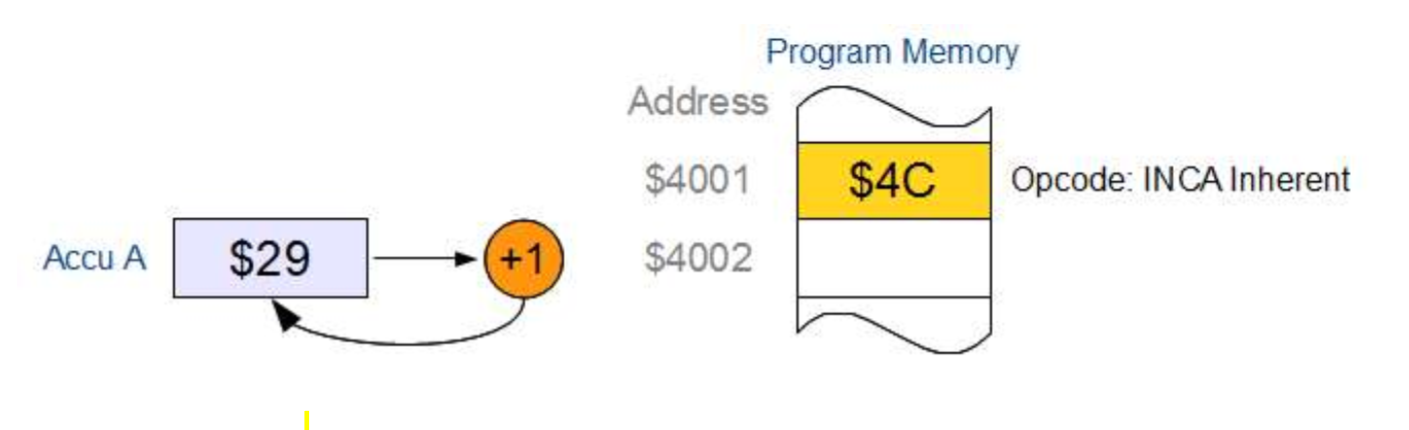
\includegraphics[keepaspectratio=true, height=10\baselineskip]{inhAdd.PNG}
	\item[Direct: ] Operands must be stored in the Direct Page (From \code{0x0000} to \code{0x00AF}) \\
		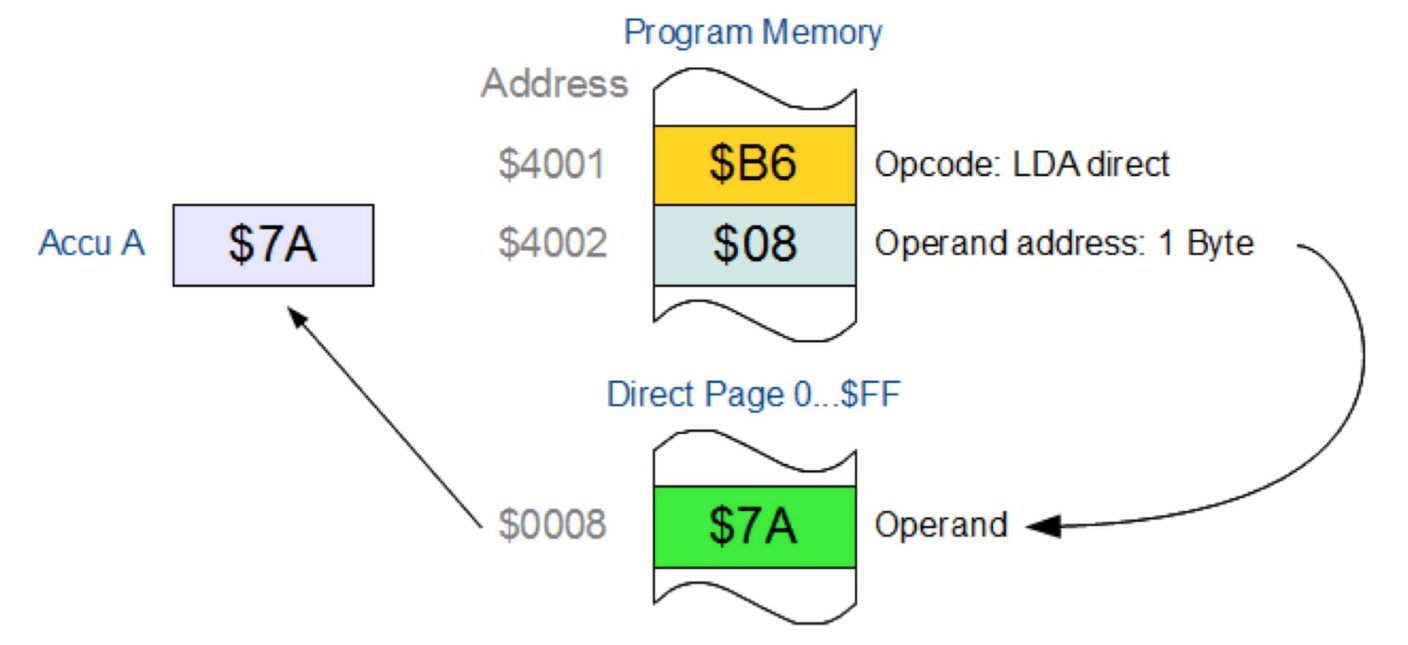
\includegraphics[keepaspectratio=true, height=10\baselineskip]{dirAdd.PNG}
	\item[Extended: ] Operand can be stored in the whole 64k Memory \\	
		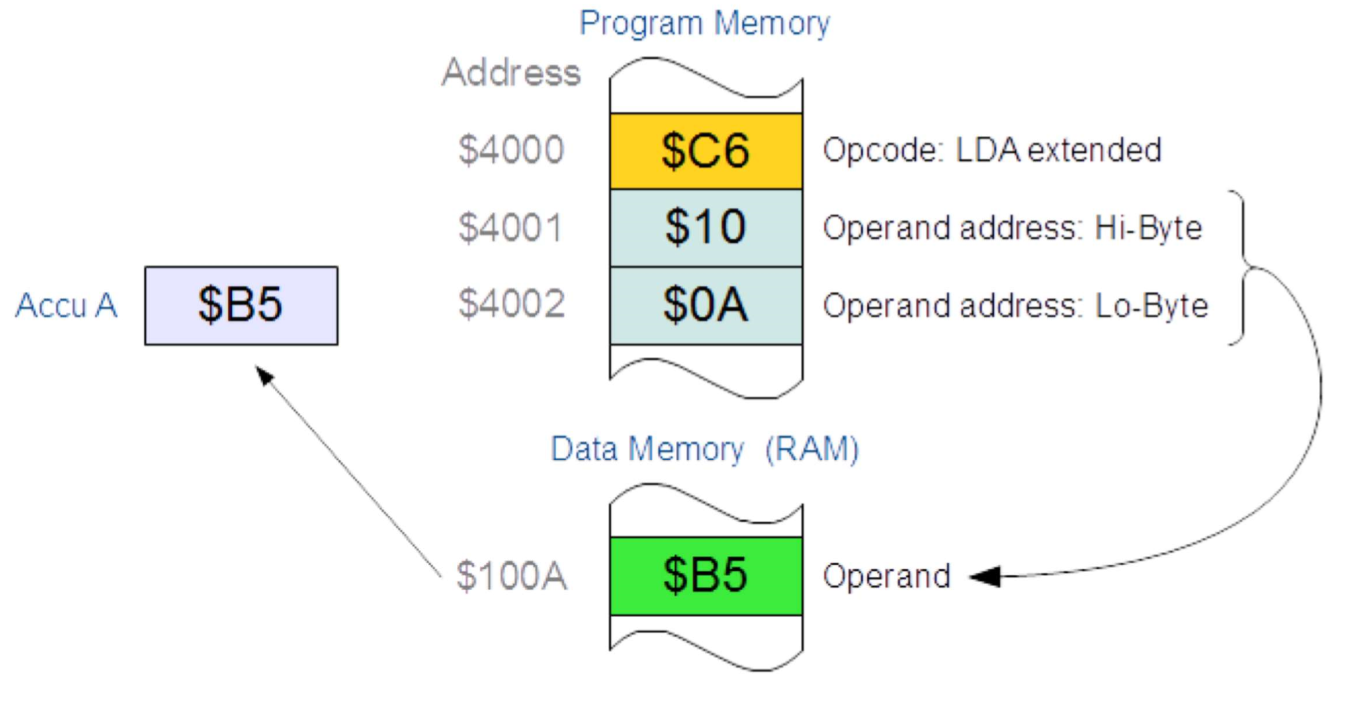
\includegraphics[keepaspectratio=true, height=10\baselineskip]{extAdd.PNG}
	\item[Indexed: ] Operand is stored in Stack Pointer or H:X Register \\
		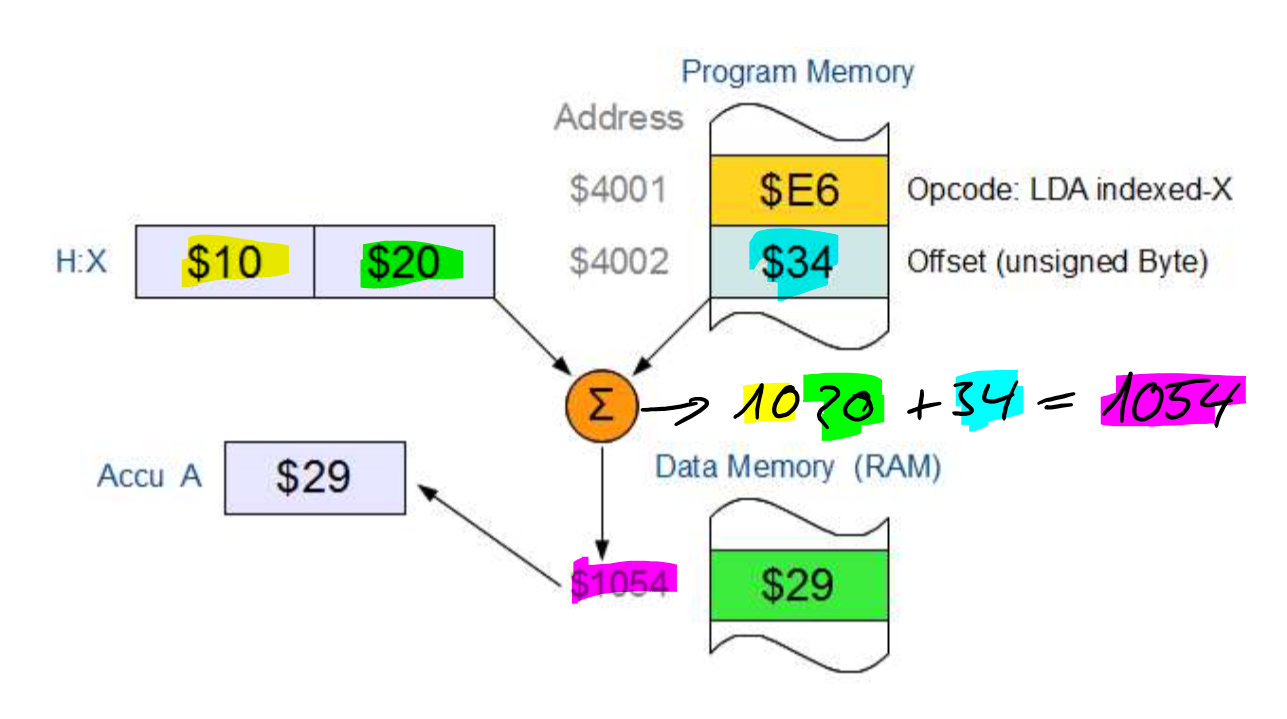
\includegraphics[keepaspectratio=true, height=10\baselineskip]{indAdd.PNG}
	\item[Relative: ] Only used with \code{BRANCH}-Instructions. Depending on outcome of the Branch \\
		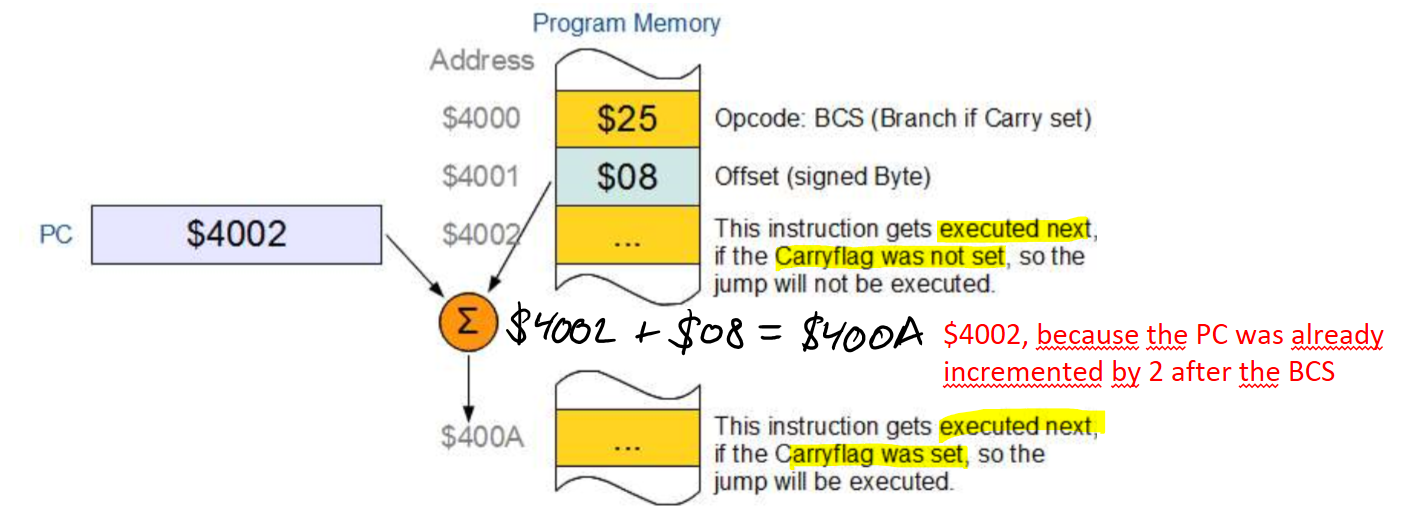
\includegraphics[keepaspectratio=true, height=10\baselineskip]{relAdd.PNG}
\end{description}

\newpage

\subsection{Assembler Programming Operations}
There are three main assembler instruction types:

\begin{itemize}
	\item Data Transport
		\subitem Load
		\subitem Store
		\subitem Transfer
		\subitem Move
	\item Operations
		\subitem Arithmetic
		\subitem Logic
		\subitem Bit-Manipulation/Masking
		\subitem Shift and Rotation
	\item Branching
\end{itemize}

\subsubsection{Data Transport}
Data Transport instructions are again divided into four subtypes

\begin{figure}[htb!]
	\centering
	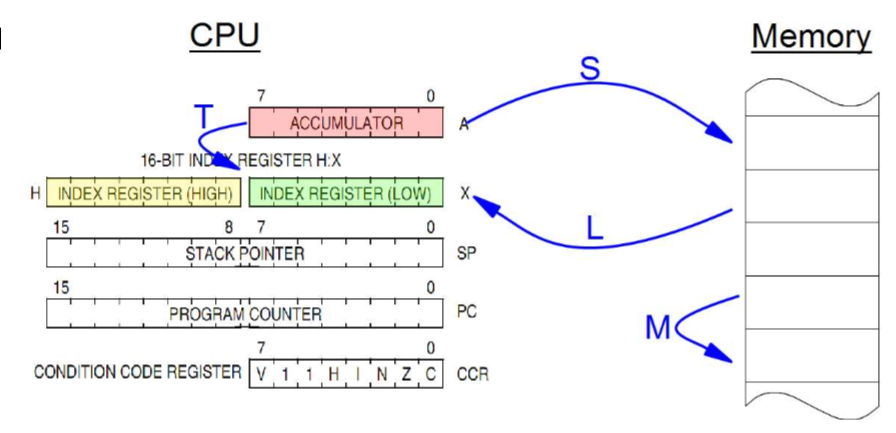
\includegraphics[keepaspectratio=true,height=15\baselineskip]{assOperations.PNG}
	\caption{Visualisation of the different data tranfers}
	\label{label}
\end{figure}

\begin{description}
	\item[Load: ] Data is moved from the memory to the CPU-Register \\
		Examples: \code{LDA, LDX, LDHX, (PULA, PULX} Stack-operations)
	\item[Store: ] Data is moved from the CPU-Register to the memory \\
		Examples: \code{STA, STX, STHX, (PSHA, PSHA} Stack-operations) 
	\item[Transfer: ] Very fast Data Transfer between CPU registers
		Examples: \code{TAP, TPA, TAX, TSX}
	\item[Move: ] Data is moved within the memory
\end{description}

\subsubsection{Arithmetic Operations}
Arithmetic operations cover the four basic mathematical operations:

\begin{description}
	\item[Addition: ] \code{ADD, ADC} (Addition with Carry Bit $\rightarrow$ supports numbers $>$ 8bit)
	\item[Subtraction: ] \code{SUB, SBC} (Addition with Carry Bit $\rightarrow$ supports numbers $>$ 8bit)
	\item[Multiplication: ] \code{MUL} Only works with unsigned numbers. Multiplies the content of the accumulator with the content of the X-register and stores the 16bit result in the X:A-registers (LSB in A, MSB in X)
	\item[Division: ] \code{DIV} Only works with unsigned numbers. Divides whatever is in the H:A-register through whatever is in the X-register. The 8bit result is stored in the accumulator. In case of an overflow or division by 0, the carry bit will be set.
\end{description}

\subsubsection{Logic and Bitmasking Operations}
Bitwise Operations change but a single bit of the operand. This can be especially useful e.g. to turn on or off LEDs, which are controlled by a register of 8 bits

\begin{description}
	\item[\code{ORA\#(B6|B3)}] \mbox{} \\
	Logical \code{OR} Operation on Bit 6 and Bit 3 $\rightarrow$ Sets \textbf{only} Bit 6 and Bit 3 in the Accumulator
	\item[\code{AND\#(B6|B3)}]\mbox{}\\
	Logical \code{AND} Operation on Bit 6 and Bit 3 $\rightarrow$ Deletes all Bits \textbf{except} Bit 6 and Bit 3
	\item[\code{BCLR n,Addr}] \mbox{}\\
	Deletes Bit n on a specific memory address
	\item[\code{BSET n, Addr}]\mbox{}\\
	Sets Bit n on a specific memory address
	\item[\code{BIT Addr}] \mbox{}\\
	\code{AND} Operation of the accumulator with the content of the address, \textit{without changing the content of either of them}
	\item[\code{CLC}] \mbox{}\\
	Clears Carry-Flag
	\item[\code{SEC}] \mbox{}\\
	Sets Carry-Flag
	\item[\code{CLI}] \mbox{}\\
	Delete Interrupt-Mask Bit ($\rightarrow$ Interrupt \textbf{enable})
	\item[\code{SEI}] \mbox{}\\
	Sets Interrupt-Mask Bit ($\rightarrow$ Interrupt \textbf{disable})
\end{description}

\newpage

\subsubsection{Shift- and Rotation Operations}

\begin{figure*}[htb]
	\centering
	\begin{subfigure}[b]{0.5\textwidth}
		\centering
		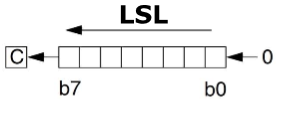
\includegraphics[keepaspectratio=true, height=5\baselineskip]{LSL.PNG}
		\caption{Logical Left-Shift}
	\end{subfigure}%
	~ 
	\begin{subfigure}[b]{0.5\textwidth}
		\centering
		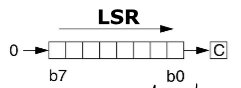
\includegraphics[keepaspectratio=true, height=5\baselineskip]{LSR.PNG}
		\caption{Logical Right-Shift}
	\end{subfigure}
	\vskip\baselineskip
	\begin{subfigure}[b]{0.5\textwidth}
		\centering
		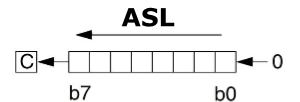
\includegraphics[keepaspectratio=true, height=5\baselineskip]{ASL.PNG}
		\caption{Arithmetic Left Shift}
	\end{subfigure}%
	~ 
	\begin{subfigure}[b]{0.5\textwidth}
		\centering
		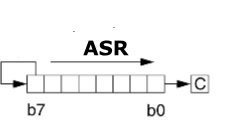
\includegraphics[keepaspectratio=true, height=7.5\baselineskip]{ASR.PNG}
		\caption{Arithmetic Right-Shift}
	\end{subfigure}
		\vskip\baselineskip
	\begin{subfigure}[b]{0.5\textwidth}
		\centering
		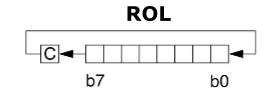
\includegraphics[keepaspectratio=true, height=5\baselineskip]{ROL.PNG}
		\caption{Rotate Left}
	\end{subfigure}%
	~ 
	\begin{subfigure}[b]{0.5\textwidth}
		\centering
		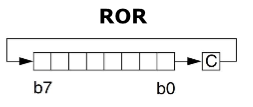
\includegraphics[keepaspectratio=true, height=7.5\baselineskip]{ROR.PNG}
		\caption{Rotate Right}
	\end{subfigure}
\end{figure*}

\noindent The Left-Shifts are an equivalent to a multiplication by two and Right-Shifts are the equivalent of a division by two:

\noindent 
$
0011'0110_{2} = 54_{10} \rightarrow LSL \rightarrow 0110'1100_{2} = 108_{10} \\
0011'0110_{2} = 54_{10} \rightarrow LSR \rightarrow 0001'1011_{2} = 27_{10}
$

\subsubsection{Branching}

\begin{tabular}{|c|c|l|}
	\hline
	\thead{Oper.}& \thead{Test} & \thead{Meaning}\\
	\hline
	\code{BEQ} & Z = 1 & Branch if equal\\
	\code{BNE} & Z = 0& Branch if not equal\\
	\hline
	\code{BCS} & C = 1& Branch if Carry\\
	\code{BCC} & C = 0& Branch if no Carry\\
	\hline
	\code{BMI} & N = 1& Branch if Negative\\
	\code{BPL} & N = 0& Branch if not Negative\\
	\hline
	\code{BGT} &$>$ & Branch if bigger (signed)\\
	\code{GHI} & &  Branch if bigger (unsigned)\\
	\hline
	\code{BGE} &$\geq$& Branch if bigger/equal (signed)\\
	\code{BHS/BCC} & & Branch if bigger/equal (unsigned)\\
	\hline
	\code{BLE} &$\leq$& Branch if lesser/equal (signed)\\
	\code{BLS} & & Branch if lesser/equal (unsigned)\\
	\hline
	\code{BLT} &$<$& Branch if lesser (signed)\\
	\code{BLO/BLS} & & Branch if lesser (unsigned)\\
	\hline
	\code{BEQ} &$=$& Branch if equal\\
	\hline
	\code{BRA} & & Branch always (Overriding SP and PC) \\
	\code{BRN} & & Branch never (Mainly used for debugging, just waits) \\
	\code{BSR} & & Brnch to subroutine (Saves SP and PC to return to main-routine) \\
	\hline
\end{tabular}
\vspace{10px}

\noindent These Branches depend on a single Bit of a memory address in the \textbf{direct pages}(\code{0x00 - 0xFF})
\begin{tabular}{|c|l|}
	\hline
	\thead{Oper.} & \thead{Meaning} \\
	\hline
	\code{BRCLR n, Addr, Label} & Branch to Label if Bit n at Address Addr is not set \\
	\hline
	\code{BRSET n, Addr, Label} & Branch to Label if Bit n at Address Addr is set \\
	\hline
\end{tabular}

\subsubsection{Comparing}
Comparing operations compare two values (kinda obvious innit?) and set the flags accordingly, but don't change the compared values:
\vspace{10px}

\noindent
\begin{tabular}{|c|l|}
	\hline
	\thead{Oper.} & \thead{Meaning} \\
	\hline
	\code{CMP opr8} & Compares content of accumulator with the 8-bit operand \\
	\hline
	\code{CPX opr8} & Compare content of X-register with 8-bit operand \\
	\hline
	\code{CPHX opr16} & Compare content of HX-register with 16-bit operand\\
	\hline
\end{tabular}

\paragraph{Example}\mbox{}\\
\begin{lstlisting}[caption={Test if a value is bigger or smaller and branch accordingly}]
LDA Op1		//Load Op1 into accumulator
CMP Op2		//Compare it to Op2 and sets Zero/Carry/Negative Flag accordingly
BMI Label	//Branch to Label if Negative flag is set (--> Op1 < Op2)
\end{lstlisting}

\newpage

\newgeometry{margin=0.5in}

\subsubsection{Flags}

\begin{figure}[htb]
	\centering
	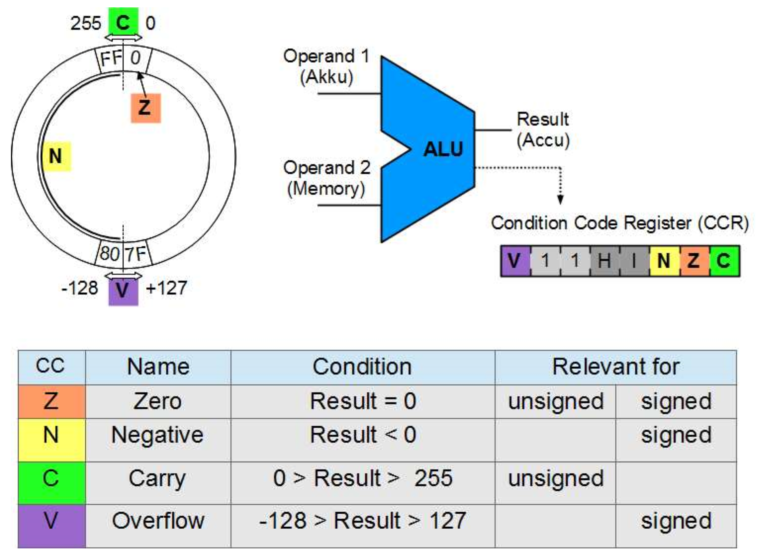
\includegraphics[keepaspectratio=true,height=19\baselineskip]{flags.PNG}
	\caption{Visualization of all supported flags}
	\label{fig:flags}
\end{figure}

\begin{figure}[htb]
	\centering
	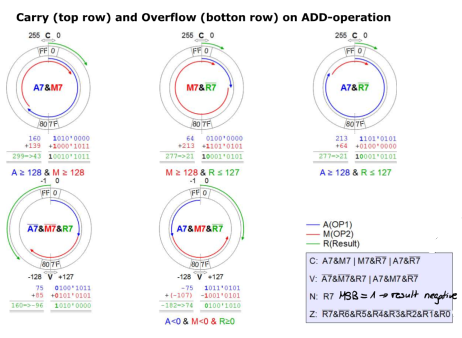
\includegraphics[keepaspectratio=true,height=19\baselineskip]{flags_add.PNG}
	\caption{Visualization of carry- and overflow-flags on Additions}
	\label{fig:flags_add}
\end{figure}

\restoregeometry
\newpage

\begin{figure}[htb]
	\centering
	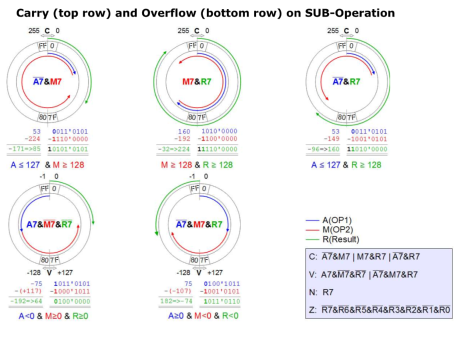
\includegraphics[keepaspectratio=true,height=20\baselineskip]{flags_sub.PNG}
	\caption{Visualization of carry- and overflow-flags on Subtractions}
	\label{fig:flags_sub}
\end{figure}

\section{Stack}
\begin{wrapfigure}[16]{R}{0.6\textwidth}
	\centering
	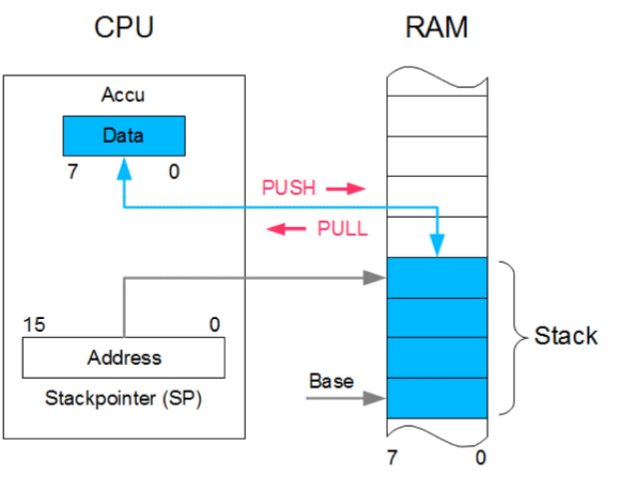
\includegraphics[keepaspectratio=true,height=18\baselineskip]{stack.PNG}
	\caption{Stack}
	\label{fig:stack}
\end{wrapfigure}

The stack is a so-called LIFO-memory (\textbf{L}ast \textbf{I}n \textbf{F}irst \textbf{O}ut), meaning whatever data is chucked on the stack last, has to be removed, before the data underneath it can be accessed.
\vspace{10px}

\noindent The Stackpointer (SP) is a pointer that always points at the next free memory place on the stack. As soon as something is pushed onto the stack (and the address the SP pointed to is therefore no longer free), it gets updated automatically. Same goes after a pull. The addresses are counted from the top of the stack, therefore the higher the stack gets, the lower the addresses.

\newpage

\begin{lstlisting}[caption={Initialization of a stack}]
Stacksize:	EQU $40			//Set the stacksize to hex 40 = 64 dec

DATA:			SECTION			//Start of DATA Section	
TofStack:	DS Stacksize-1	//Reserve memory for the stack
BofStack:	DS 1

PROGRAM:		SECTION
				//Initializing SP(+1, bc SP always points to the first free address)
				LDHX #(BofStack+1)	//LDHX = Load value into H:X-Register
				TXS		//Transfer SP to H:X Register
			
				PSHA	//Push accumulator to Stack
				PSHX	//Push X-register to Stack
				
				//Important! Reverse order bc of LIFO
				PULX	//Pull X-Register from Stack
				PULA	//Pull accumulator from Stack
\end{lstlisting}

\chapter{C}

\end{document}
